% Thesis Introduction

\chapter[Introduction]{Introduction}
\label{chap-intro}

In the field of robotics, manipulation is an important aspect to all robotic systems. Regardless of its form factor, a robot's means of manipulation is an important factor that affects how it is controlled, and what applications it can be applied to. In this thesis, the manipulation systems of three different robots are presented and analyzed. The first robot prestented, a magnetic manipulator cooled with liquid nitrogen, deals with a millimeter scale robot whose position and orientation are controled by three pairs of electromagnetic coils placed orthogonal to each other. In this system, the manipulators are the 6 coils and their magnetic fields. In order to increase the strength of the fields in this system without using iron cores, each coil was cooled to cryogenic temperatures.  By cooling the coils and reducing their resistances, more current can be driven into the coils and increase their fields proportionally.  Fig. \ref{MagTopPic} shows a top view of the system with the top coil taken out.  The second system presented in this thesis is a two dimensional manipulator system similar to the the first, but with a smaller workspace, and using solid iron cores to concentrate the magnetic field. This system was used to implement an algorithm to move a pair of 'robots' to predefined goal locations by taking advantage of the cavity's geometry, surface friction and global inputs to both robots. Fig. \ref{Intestine} shows one of the cavities, the phantom intestine model, used to test the algorthm.  For the third and final system, the manipulator considered is a five degree of freedom robotic arm. The arm originally comes without any sensors on its joints, but through the additon of several fabricated parts and sensors, the arm's manipulability and functionality are increased significantly. 


\begin{figure}
\centering
	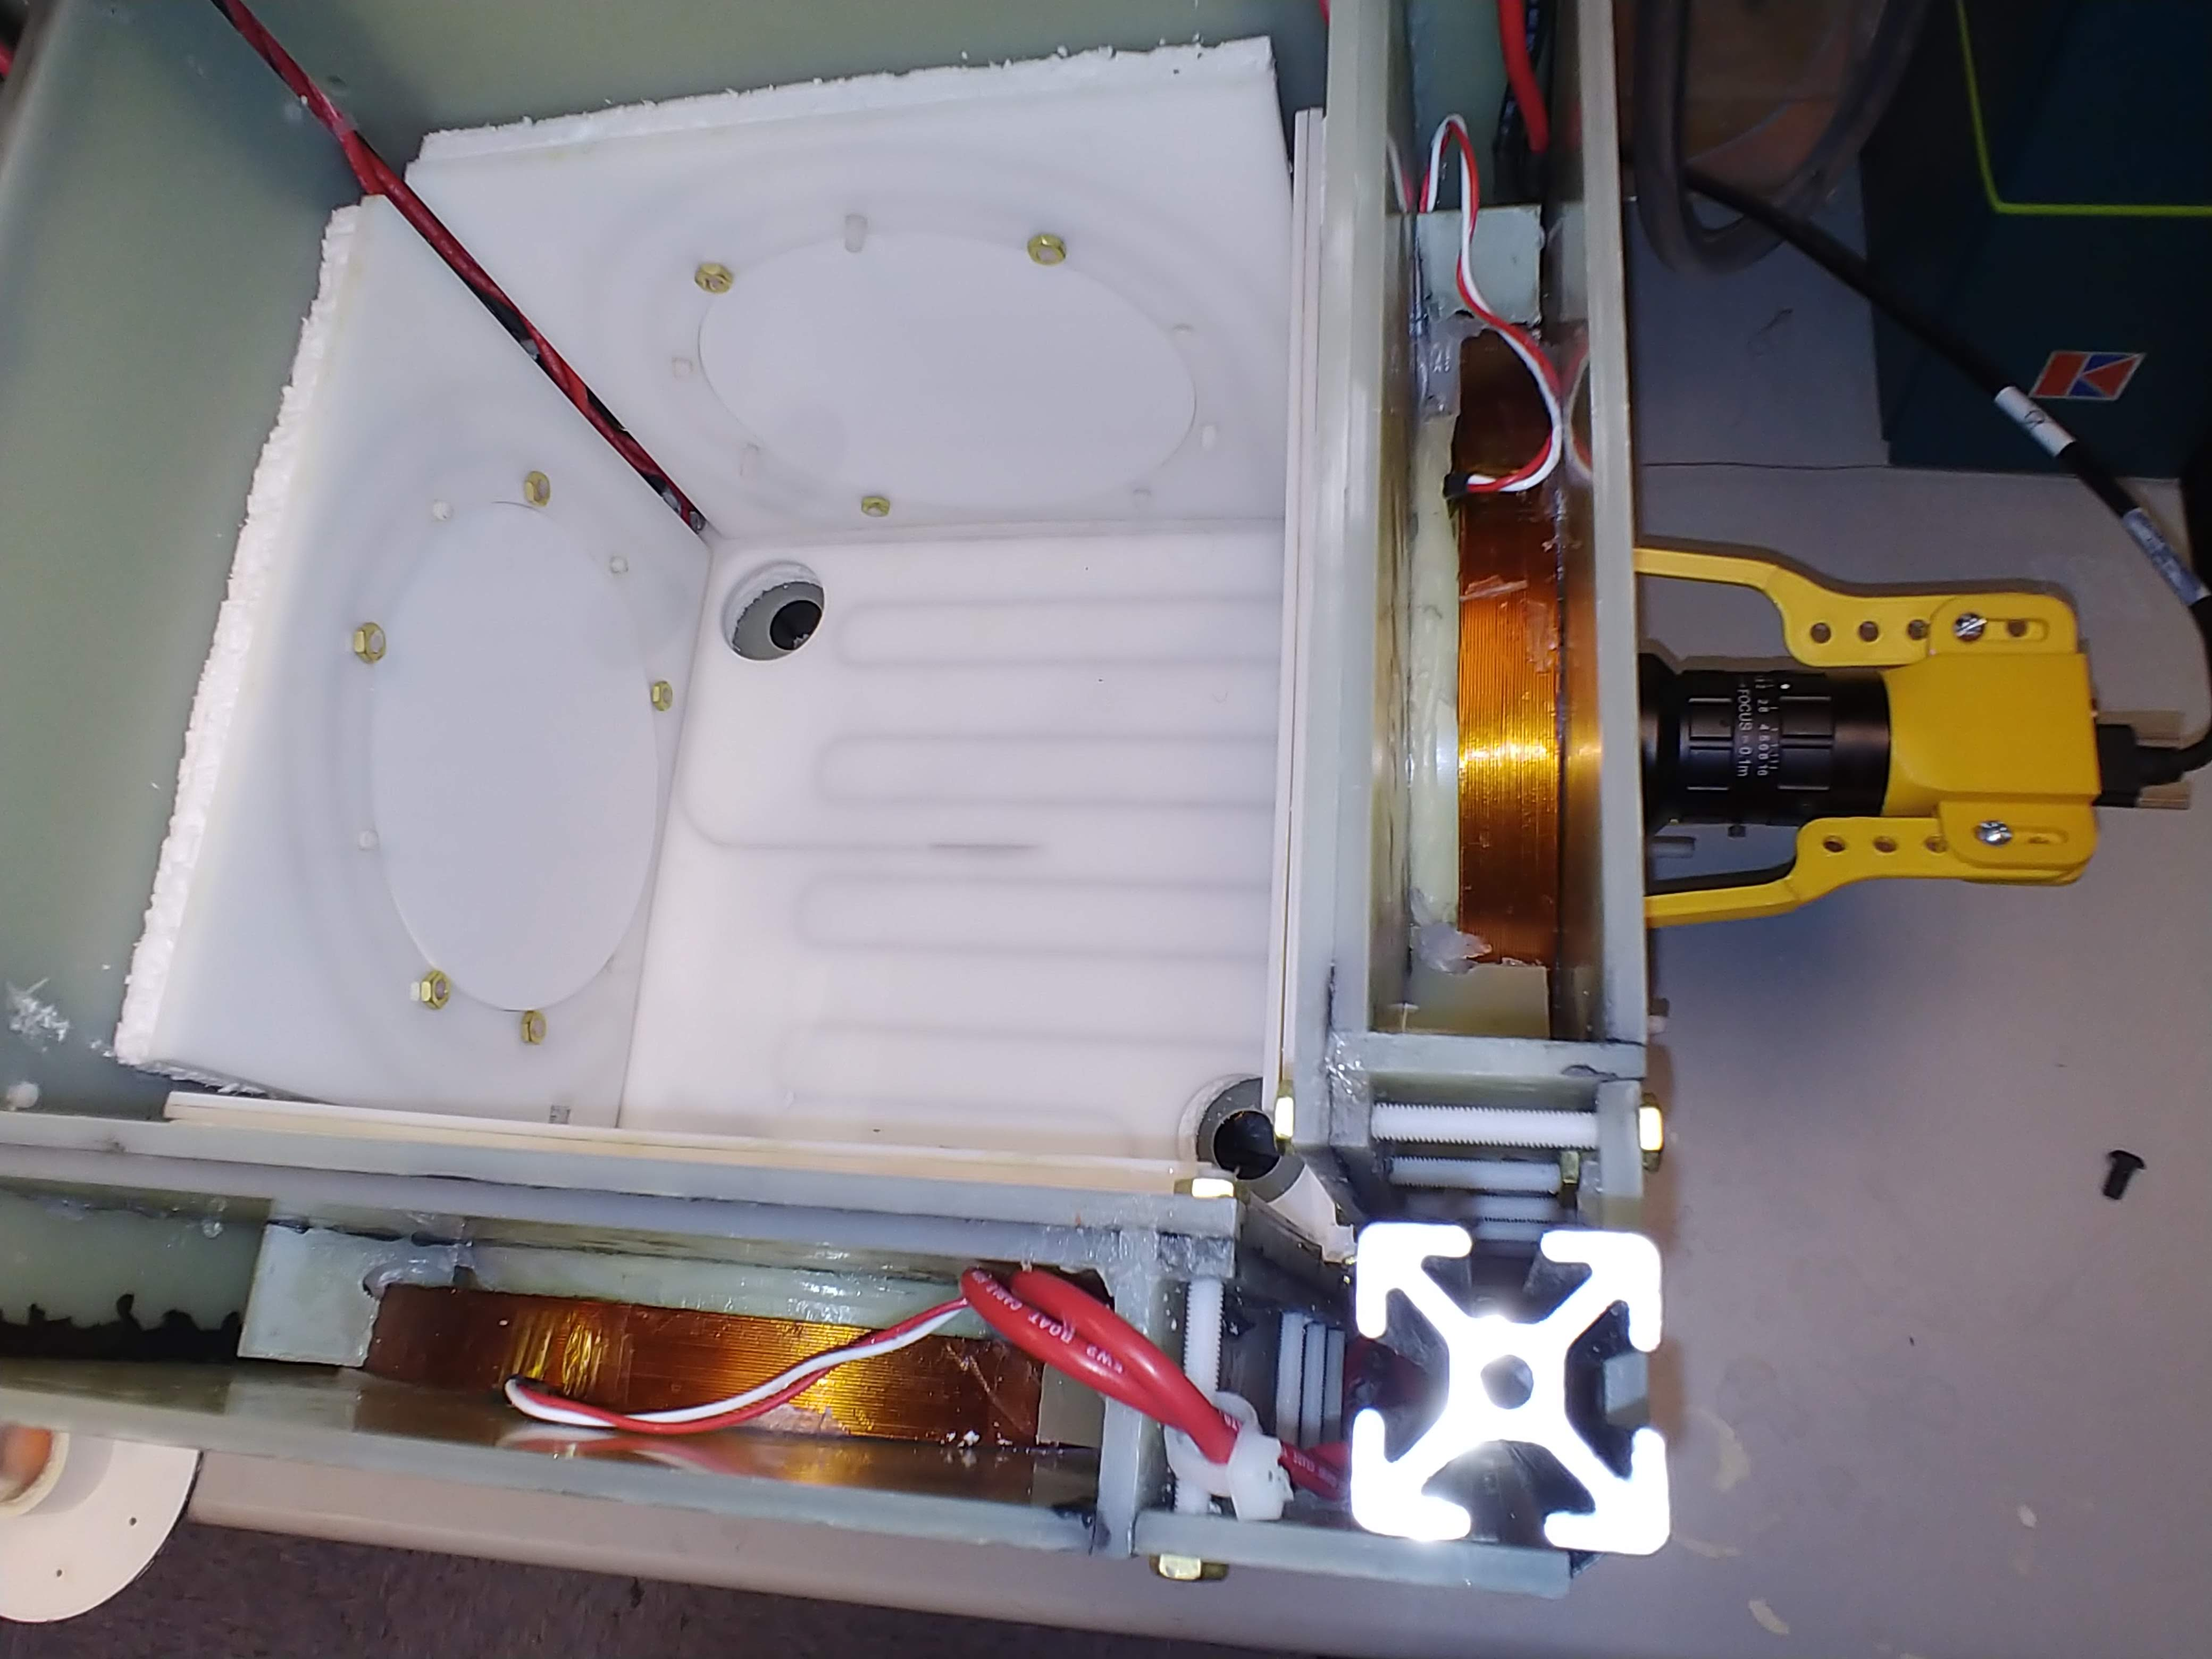
\includegraphics[width=0.7\columnwidth]{Magsystemtop.jpg}
	\caption{Top view of the magnetic manipulator, showing  two of the side coils and one of the camera sensors}.
	\label{MagTopPic}
\end{figure}  
\begin{figure}
\centering
	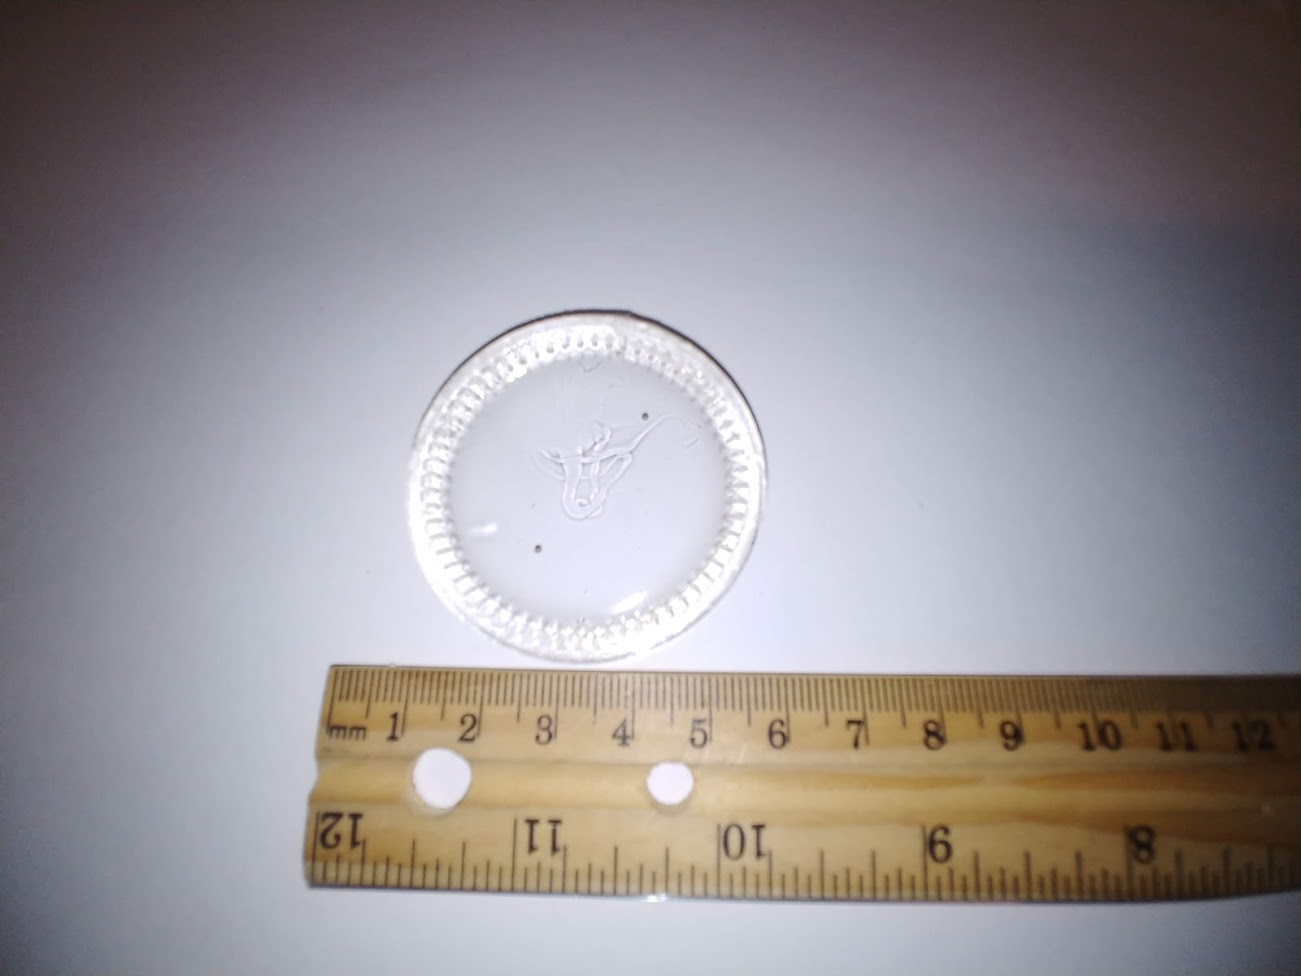
\includegraphics[width=0.7\columnwidth]{Phantomintestine.jpg}
	\caption{The phantom intestine model, used to simulate the small intestine of a cow along with its villi}.
	\label{Intestine}
\end{figure} 